% Chapter 1

\chapter{Introduction} % Main chapter title

\label{Chapter1} % For referencing the chapter elsewhere, use \ref{Chapter1} 

\lhead{Chapter 1. \emph{Introduction}} % Change X to a consecutive number; this is for the header on each page - perhaps a shortened title

%----------------------------------------------------------------------------------------
\section{\textbf{Wireless Applications}}

Our modern society heavily depends on the wireless spectrum for communication purposes.
Telecommunications, financial transactions, health services, military services, environment
surveillance, entertainment, and social activities are just several of the numerous applications
examples in our daily life.
\begin{figure}
    \centering
    \includegraphics[width=1\linewidth]{Figures/chapter1/Forecast year-on-year mobile data traffic growth rates by region 2022–2029.png}
    \caption{Forecast year-on-year mobile data traffic growth rates by region 2022–2029 \cite{ref26}}
    \label{fig:forecast1}
\end{figure}

Forecast year-on-year growth rates of mobile data traffic. The growth rate for mobile data is expected to slow every year between 2022 and 2029 in all regions. The region, which includes India, Nepal and Bhutan, consistently shows a higher growth rate than the global average.
All lines are trending downwards, indicating that while data usage is still growing, it is growing at a slower pace each year (Figure: \ref{fig:forecast1}).  

\begin{figure}
    \centering
    \includegraphics[width=1\linewidth]{Figures/chapter1/Forecast yearly net added mobile data traffic 2022–2029.png}
    \caption{Forecast yearly net added mobile data traffic 2022–2029 \cite{ref26}}
    \label{fig:forecast2}
\end{figure}

 Forecast yearly net added mobile data traffic.The total amount of new mobile data traffic added each year is forecast to increase steadily from 2022 to a peak in 2027. After 2027, the amount of newly added traffic is expected to decrease slightly. The bars get taller until 2027, meaning that the sheer volume of new data added to networks will continue to grow for the next few years (Figure: \ref{fig:forecast2}).

\section{\textbf{Cognitive Radio Network(CRN)}}
With the rapid development in communication applications the spectrum becomes more congested and also the need for data rate increased. The radio spectrum is a limited resource and the service is allocated by fixed spectrum assignment. So some frequencies are heavily used, and other bands are weakly used.
The number of devices that use unlicensed spectrum is growing, which indicates an increase in spectrum demand. So spectrum scarcity is a major issue faced by wireless networks. In order to overcome this issue, dynamic spectrum access (DSA) is introduced, which improves the spectrum efficiency. In DSA the unlicensed systems are allowed to use the licensed bands without interfering with the existing user. So the weakly used spectrum can be used by other users. In Figure:\ref{fig:crn} Cognitive Radio (CR)
uses dynamics spectrum allocation which provides higher bandwidth and efficient spectrum usage. CR enables reuse of the licensed spectrum in an unlicensed manner i.e., it opens the licensed bands to unlicensed users to use them without causing any interference to the licensed user. Radio sensing, self adaptation and dynamic spectrum sharing are the abilities of CR. Spectrum under utilization and spectrum scarcity can be mitigated by an efficient spectrum usage of CR \cite{ref2}. 

Key features of Cognitive Radio include:
    Radio Sensing,
    Self-Adaptation
    and Dynamic Spectrum Sharing




\subsection{\textbf{Overview of CR and CRN}}

CR stands for Cognitive Radio and CRN stands for Cognitive Radio Networks \cite{ref1}. These are advanced wireless communication technologies that aim to improve spectrum utilization and efficiency.

\textbf{Cognitive Radio (CR)}

    A radio that can intelligently sense its environment, detect available spectrum opportunities, and dynamically adapt its parameters (e.g., frequency, power, modulation) to efficiently utilize the spectrum.
    Key features are 
        Spectrum Sensing: The ability to detect unused or underutilized spectrum bands.
        Spectrum Decision: The ability to make intelligent decisions about which spectrum bands to use.
        Spectrum Access: The ability to dynamically access and utilize available spectrum bands.
    Benefits are  
        Improved spectrum utilization, Reduced interference, Increased network capacity, Enhanced flexibility and adaptability. \\ 

\textbf{Cognitive Radio Networks (CRN)}

\begin{figure}
    \centering
    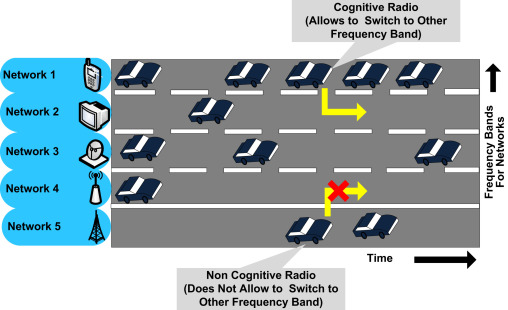
\includegraphics[width=0.8\linewidth]{Figures/chapter1/CRN overview.jpg}
    \caption{CRN overview \cite{ref27}}
    \label{fig:crn}
\end{figure}

A network of cognitive radios that can collaborate and coordinate their spectrum access to optimize overall network performance.
    Key features \cite{ref1} are Cooperative Spectrum Sensing: Multiple cognitive radios can collaborate to improve spectrum sensing accuracy and coverage.
        Spectrum Sharing: Cognitive radios can share spectrum resources among themselves and with other networks.
        Dynamic Spectrum Management: CRNs can dynamically manage spectrum access to optimize network performance and meet changing demands.
    Benefits are : Improved spectrum efficiency, Enhanced network reliability, Increased network capacity and Better quality of service
 
\subsection{\textbf{Functions of CRN}}

Cognitive Radio Networks (CRNs) leverage advanced technologies to optimize the use of the radio frequency (RF) spectrum, addressing the challenges of spectrum scarcity and inefficiency through several key functional areas \cite{ref1}. The foundational function is spectrum sensing, which enables cognitive radios to detect unused portions of the spectrum, often referred to as spectrum holes or white spaces, allowing them to identify which channels are occupied by primary users and which are available for secondary users \cite{ref1,ref6}. Various sophisticated techniques are employed for spectrum sensing, including energy detection, matched filtering, and cyclostationary feature detection, each offering distinct advantages and limitations \cite{ref4,ref6}. Once available spectrum is identified, spectrum management becomes crucial as cognitive radios must effectively select the best available channel based on communication requirements such as bandwidth, signal quality, and interference levels, ensuring dynamic adaptation to changing network conditions and user demands \cite{ref1,ref3}.

The operational capabilities of CRNs are further enhanced by spectrum mobility and sharing functions, which are essential for maintaining service quality while adhering to regulatory constraints. Since cognitive radios operate as secondary users with lower priority, spectrum mobility enables them to seamlessly transition to alternative available channels when primary users are detected, maintaining ongoing communications without disruption \cite{ref1,ref3}. In multi-user environments, spectrum sharing coordinates access among various cognitive radios to ensure fair usage and minimize interference through sophisticated scheduling algorithms and protocols \cite{ref1,ref3}. The cognitive capability encompasses the fundamental ability to perceive, learn, and adapt to environmental changes, enabling informed decision-making for channel selection and usage \cite{ref1,ref2}. Additionally, reconfigurability allows cognitive radios to dynamically adjust transmission parameters such as frequency, power, and modulation schemes based on detected spectrum conditions, while learning and adaptation capabilities enable performance enhancement over time through experience-based strategy optimization and historical data analysis \cite{ref1,ref3,ref9,ref19}. These functions collectively enable CRNs to utilize the RF spectrum more efficiently, improving overall communication quality and expanding network capacity to support growing numbers of connected devices and applications \cite{ref1,ref2,ref3}.


\subsection{\textbf{Cognitive cycle}}

The cognitive cycle is a fundamental concept in Cognitive Radio Networks (CRNs), representing the iterative process through which cognitive radios (CRs) adaptively manage spectrum resources as illustrated in Figure \ref{fig:cr_cycle} \cite{ref1,ref3}. This comprehensive cycle consists of four interconnected key functions that work together to enable intelligent spectrum management. The initial phase, spectrum sensing, involves continuous monitoring of the radio environment to detect the presence of primary users (PUs) and identify available spectrum bands, which is crucial for avoiding interference with licensed users and ensuring efficient spectrum utilization \cite{ref1,ref4,ref6}. Following the sensing phase, spectrum decision requires cognitive radios to analyze the sensed data and make intelligent choices about which spectrum band to utilize, considering factors such as channel quality, secondary user requirements, and potential interference levels \cite{ref1,ref3}.

\begin{figure}
    \centering
    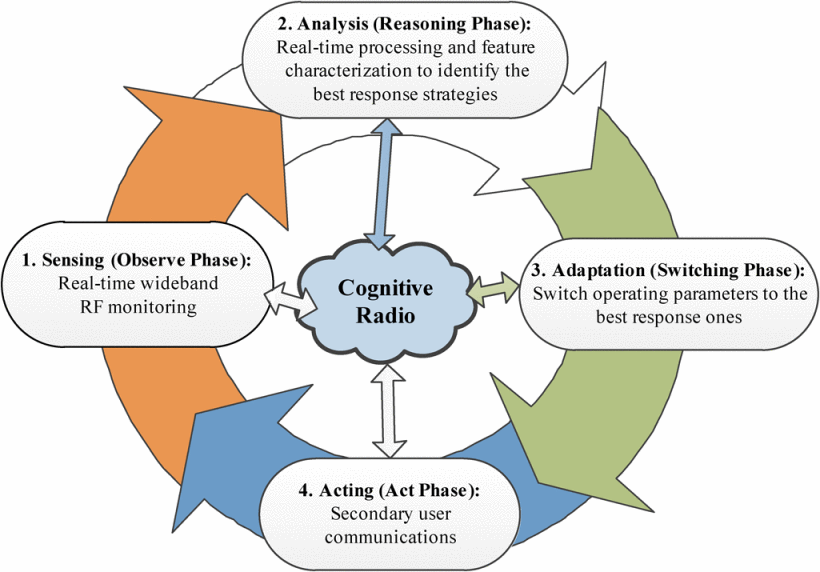
\includegraphics[width=0.8\linewidth]{Figures/chapter1/cr_cycle.png}
    \caption{Cognitive Cycle \cite{ref29}}
    \label{fig:cr_cycle}
\end{figure}

The operational phases of the cognitive cycle ensure seamless spectrum access and dynamic adaptation to changing radio environments. Once a spectrum decision is made, spectrum sharing becomes essential as cognitive radios must negotiate access to the selected spectrum band through coordination with other cognitive radios, ensuring spectrum utilization without causing disruption to primary users or other secondary users \cite{ref1,ref3}. The final phase, spectrum mobility, enables cognitive radios to dynamically switch channels as the radio environment changes, allowing them to maintain communication links while avoiding interference with primary users that may become active \cite{ref1,ref3}. This iterative cognitive cycle enables CRs to continuously adapt to the dynamic nature of wireless communication, optimizing spectrum usage and enhancing overall network performance through intelligent, real-time decision-making processes \cite{ref1,ref3}.

%----------------------------------------------------------------------------------------
\section{\textbf{Architecture of CRN}}

The architecture of Cognitive Radio Networks (CRNs) is designed to facilitate intelligent spectrum management and enhance communication efficiency through a sophisticated framework of interconnected components \cite{ref1,ref2}. As illustrated in Figure \ref{fig:CRN_arc}, the core of this architecture is the cognitive engine, which serves as the brain of the CR, processing environmental information and making intelligent decisions based on the cognitive cycle \cite{ref1}. This cognitive engine incorporates advanced machine learning algorithms to continuously improve its decision-making capabilities over time, enabling adaptive and intelligent spectrum management \cite{ref9,ref19}. The spectrum sensing module works in conjunction with the cognitive engine to detect the presence of primary users and identify idle channels through various sophisticated techniques, including energy detection, matched filtering, and cyclostationary feature detection, ensuring accurate spectrum awareness \cite{ref4,ref6,ref11}.

\begin{figure}[ht]
    \centering
    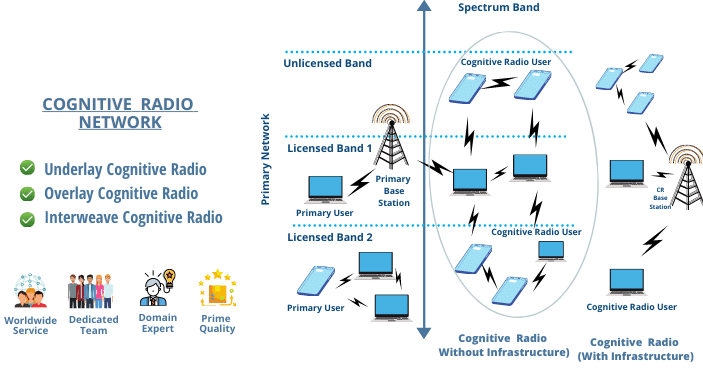
\includegraphics[width=\linewidth]{Figures/chapter1/CRN-Thesis.png}
    \caption{CRN Environment \cite{ref28}}
    \label{fig:CRN_arc}
\end{figure}

The operational efficiency of CRNs is further enhanced by the spectrum management module, which allocates spectrum resources based on user demands and environmental conditions while ensuring efficient utilization that balances the needs of both primary and secondary users \cite{ref1,ref3}. The communication module facilitates reliable data transmission over the selected spectrum, ensuring efficient communication between devices throughout the network \cite{ref2}. Given the inherent vulnerabilities of CRNs to various security threats, a robust security framework is integrated into the architecture as an essential component, incorporating mechanisms for detecting and mitigating attacks such as Primary User Emulation Attacks (PUEA) and Spectrum Sensing Data Falsification (SSDF) \cite{ref1,ref7,ref25}. Overall, this comprehensive architecture enables CRNs to support dynamic spectrum access while maintaining reliable communication and robust security measures \cite{ref1,ref25}.

%----------------------------------------------------------------------------------------
\section{\textbf{Security Issues in CRN}}

Cognitive Radio Networks (CRNs), while designed to address spectrum scarcity through dynamic spectrum access, introduce significant security vulnerabilities that can severely impact network performance and reliability \cite{ref25}. The most critical threat is the Primary User Emulation Attack (PUEA), where malicious users mimic the behavior of primary users, forcing legitimate secondary users to vacate spectrum bands and leading to inefficient spectrum utilization \cite{ref7}. This attack essentially functions as a denial of service mechanism, causing secondary users to experience increased call drop rates, communication delays, and severe quality of service degradation \cite{ref1}. Additionally, Spectrum Sensing Data Falsification (SSDF) attacks exploit vulnerabilities in collaborative spectrum sensing by manipulating sensing data to mislead secondary users about spectrum availability, further compromising network integrity \cite{ref6}.

The dynamic nature of CRNs creates additional security challenges that extend beyond traditional wireless network threats. Control channel vulnerabilities pose particular risks, as compromise of the common control channel (CCC) used for exchanging control messages can lead to complete network outages, rendering entire CRN systems inoperable \cite{ref25}. The continuous requirement for secondary users to estimate primary user parameters during dynamic spectrum access exposes them to eavesdropping and other sophisticated attacks \cite{ref3}. These security issues can be broadly categorized into infrastructure-based attacks (such as PUEA and SSDF) and infrastructure-less attacks (including greedy secondary user behaviors), each presenting unique challenges that require comprehensive security frameworks to ensure reliable and secure cognitive radio operations \cite{ref1,ref7}.
